\section{Funktionsumfang der Beispiel Anwendung}
Grundsätzlich wurde beim Entwurf des Funktionsumfang versucht, die typischen Funktionalitäten von Applikationen abzubilden. Eine Befragung mobiler Anwendungsentwickler durch JetBrains ergab, dass die wichtigsten Funktionen Datenspeicherung, Kommunikation über Netzwerk, Medienanzeige, Status und Navigationsmanagment, Datensynchronisierung, Dateien lesen/schreiben, Sicherheit, Bezahlung, Berechnungen und Machine Learning sind\cite{JetBrains_miscellaneous_2021}. Natürlich sind gerade der letzte Punkt oder die Bezahlung eine sehr Anwendungsfallspezifische Sache, jedoch gibt es einem einen guten Kompass was eine App so grundlegend Abzudecken hat.
Um den Arbeitsaufwand realistisch zu halten und trotzdem aber einige der oben genannten Parameter abzudecken, ist die Implementierung wie im Folgenden beschrieben eingeschränkt:

Allgemein soll eine App gebaut werden, die wie bereits erwähnt sich an einer bestehende Webanwendung orientiert und einen Teil der Funktionalität durch die Programmierung abbilden soll. Des weiteren wird eine GraphQL-Schnittstelle genutzt um die Daten der Webanwendung zu Nutzen. 

\subsection{Nativer und Cross-Plattform Ansatz}
Bei der Nativen und der Multi-Plattform Applikation bilden wir den in Abbildung \ref{fig:pageflow} dargestellten Ablauf ab. Dabei sind diese komplett durch in der Applikation implementierten Seiten dargestellt. Diese sind eine Startseite, eine Login- , Profil- , Kommunikations- und einer Chatseite. Dadurch schaffen wir es, die oben genannte Aspekte bis auf Bezahlung und Machine Learning, die für diese Applikation auch kein Anwendungsfall haben, größtenteils abzudecken. Denn durch den Login etwa erfüllt die Applikation teilweise die Bereiche Sicherheit, Statusmanagment, Daten lesen/schreiben und Kommunikation über Netzwerk. 

\begin{figure}[ht]
  \centering
  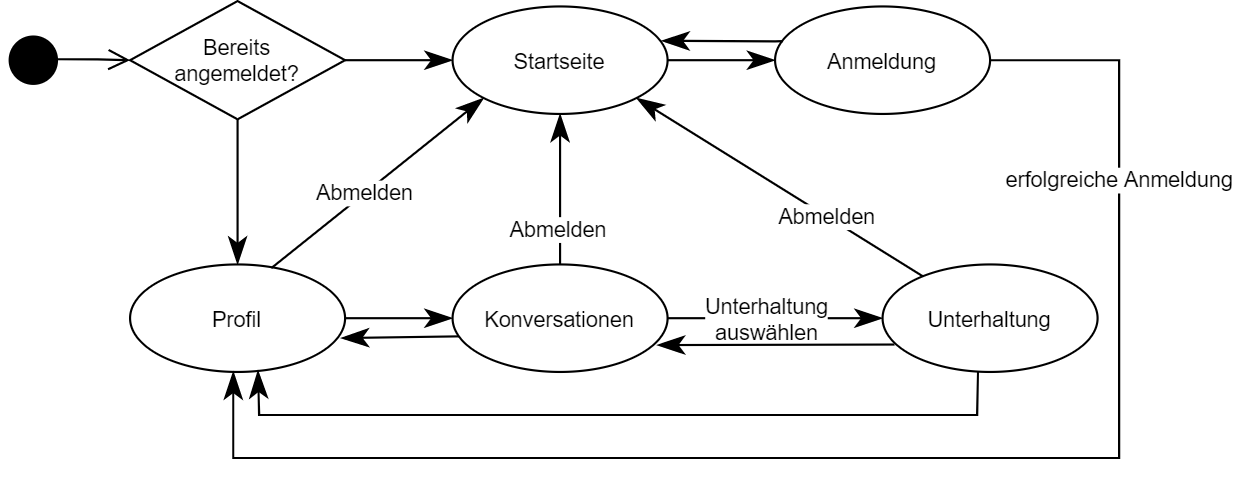
\includegraphics[height=7cm,keepaspectratio]{images/Pageflow_native_flutter.png} 
  \caption{Verbindungen zwischen den Seiten der implementierten Applikation beim nativen Ansatz und dem Multi-Plattform-Ansatz}
  \label{fig:pageflow}
\end{figure}

Der genaue Ablauf der App ist, dass der Nutzer die App öffnet. Ist er bereits eingeloggt, wird er automatisch auf die Profil Seite übergeleitet, auf der seine eigenen Sachen angezeigt werden. Ist er nicht angemeldet, so landet er auf einer Startseite/ Willkommensseite, auf der einige Sachen über das Projekt erklärt werden und kann dann zu der Loginseite weiter, von der er nach erfolgreichem Anmelden zu der bereits erwähnten Profilseite kommt. Über einen Knopf in der Menüleiste der App kann der eingeloggte Nutzer auf die Konversationsseite wechseln. Hier wird im eine Liste an Konversationen angezeigt, an denen er beteiligt ist. Nun kann er durch einen Klick auf eine Unterhaltung zu dem Chat wechseln, kann hier die bereits bestehenden Nachrichten lesen und neue Nachrichten abschicken. Mit der Zurück-Taste kann er dann wieder zu der Konversationsseite zurückkehren oder über einen Klick auf das Logo zur Profilseite zurückkehren. Als letztes ist in der Menüleiste noch ein Knopf mit dem Text "Abmelden". Wenn man diesen drückt, werden die gespeicherten Zugangsdaten gelöscht und der Nutzer somit abgemeldet. Nach erfolgreichem Abmelden wird er dann wieder zu der Startseite zurückgeführt.

\subsection{Hybrider und Gemischter Ansatz}
Bei den hybriden Absätzen wird die Website mit in die Applikation eingebunden. Je nach Art des hybriden Ansatzes unterscheidet sich hier der Umfang und Ablauf. So wird etwa bei den in Kapitel 4.2 vorgestellten Implementierungen unter Umständen nur die Website in einer Applikation angezeigt. In Kapitel 4.4 jedoch wird die oben erklärte Implementierung mit einer Anzeige der Website gemischt. So wird im vergleich zu Abbildung \ref{fig:pageflow} die Startseite durch die Startseite der Webseite ersetzt. Zusätzlich dazu wird durch eine veränderte Navigation über ein Seitenmenü die zusätzliche durch die Webanwendung verfügbare Funktionalität durch Verlinkung hinzugefügt. Etwa kommen hierdurch eine Übersicht der Kreise in denen der Nutzer Mitglied ist oder eine Liste der Gegenstände die man ausleihen kann hinzu.


